%% Lee
%% In dissertation, change 
%    section* to chapter 
%    subsection* to section
%    subsubsection* to subsection

\chapter{Artificial Neural Networks}
%\section{Artificial Neural Networks}
\label{sec:chap-two}

Recently, there has been much interest in the use of artificial neural networks in systems that employ tasks such as image recognition\cite{krizhevsky2012imagenet}, text recognition\cite{qiu2013parallel} and game playing\cite{maddison2014move}.
In particular, in the field of image recognition these artificial neural network models have demonstrated superior performance
over other state-of-the-art technology\cite{krizhevsky2012imagenet}.
%There is reason to believe 
These artificial neural networks will continue to be applied to numerous other areas such as voice recognition, text recognition, 
face recognition and autonomous control.

Artificial neural networks (\ac{ann}) take their inspiration from neuron behavior observed in the mammalian brain, although implementations are simplifications of what actually exists in the brain.

The mammalian neuron is a cell that receives input and generates output in the form of electrical and chemical processes.
The neuron has a cell body (or soma), a group of dendrites which provide the inputs from other cells, a cell body, an axom which generates the output signals, and the axom terminals which are the outputs of the cell.
The connection from a cells output, or axom terminal to another cells input, or dendrite is known as a synapse. 
The connection in the synapse is a chemical process stimulated by electrical impulses.
The neuron can be seen in figure \ref{fig:neuron}.

The connection from one cell to another has both an associated delay and a strength. The strength of the connection can be influenced by the size of the pre-synaptic neuron spike or by the pre-synaptic neuron generating a series of spikes rather than a single spike.

\begin{figure}[!t]
% the [] contains position info e.g. [!t] means here
\centering
\captionsetup{justification=centering}
\captionsetup{width=.9\linewidth}
\centerline{
\mbox{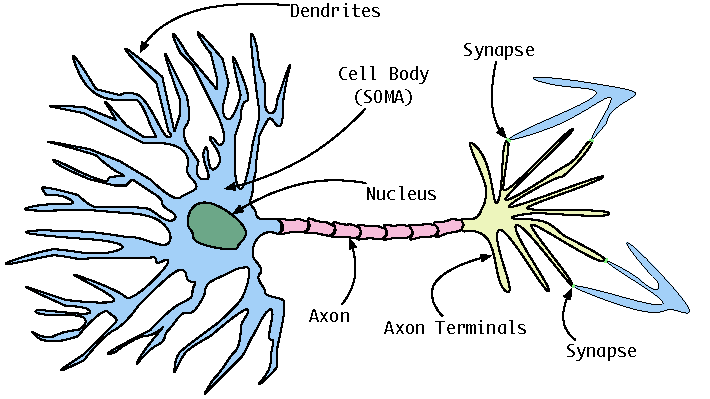
\includegraphics[width=4.0in]{Neuron.pdf}}
}
\caption{Artists impression of a Mammalian Neuron}
\label{fig:neuron}
\end{figure}



\iftrue
So it is known that mammalian neurons generate "spikes" in response to inputs which for humans include sight, touch, sound etc.. This spiking behavior is often referred to as the neuron being activated.
When these neurons are activated, their spikes propagate to other neurons. Under certain conditions, the combination of the various inputs to a neuron cause it to activate. 
A particular neuron may have many hundreds, perhaps thousands of other neurons connected to its "input".
These input neurons are referred to as pre-synaptic neurons. These pre-synaptic neurons may provide input to many neurons which are referred to as post-synaptic neurons.
A particular neuron can get activated by a particular arrival pattern of pre-synaptic neuron spikes or simply by the intensity of the pre-synaptic spikes. 

The spiking behavior of a neuron also varies and many spiking profiles have been observed, including single spikes, groups of spikes and repetitive spiking. 
It is believed that information is carried in the delay and strength of the connections and how pre-synaptic neurons combine to cause a neuron to activate.
In simple terms, if a neuron is activated by its pre-synaptic neurons, then the activation of the neuron means a pattern has been detected which will influence a reaction.
In mammalian terms, that might be the detection of a threat from both smell and sight neurons and the reaction is to control muscles resulting in flight.


The various chemical and electrical processes that result in the generation and propagation of these neuron spikes is beyond the scope of this dissertation, but how neurons and networks of neurons are artificially emulated is what we will discuss next.


%\section[NnSP]{NnSP{\cite{esmaeilzadeh2005nnsp}}}
\section[ANN Overview]{ANN Overview}
\label{sec:ANN Overview}

When modeling these neurons in artificial neural networks, the neuron models either generate actual spikes similar to actual neurons or
produce a value which is proportional to the rate at which spikes occur.
These artificial neural networks can be categorized as rate-based coded or spike time coded neurons.


When used in networks of neurons, both model types employ a connection weight between the pre and post-synaptic neuron, however, the spiking neuron network also introduces a time delay associated with the connection.

The spiking neuron model is characterized by:

\begin{outline}
  %\setlength{\baselineskip}{10pt}
  %\setlength{\itemsep}{12pt}
  %\setlength{\partopsep}{0pt}
  %\setlength{\parskip}{0pt}
  %\setlength{\parsep}{0pt}
  %\setlength{\topsep}{0pt}
  %\setlength{\itemindent}{\leftmargin}
  %\setlength{\leftmargin}{0pt}
        \1 Connections between neurons have both a strength and a delay
          \2 The pre-synaptic neuron output is multiplied by the connection weight and delayed
        \1 The weighted inputs from all pre-synaptic neurons are accumulated
        \1 The accumulated inputs drives an activation function
          \2 the activation function $f(x)$ is a spiking model is based on differential equations
          \2 many models have been proposed with varying levels of complexity
            \3 examples are:
              \4 Leaky integrate and fire
              \4 Izhikevich \cite{Iz2005} (see \fref{fig:Izhikevich Model})
         
\end{outline}

The Rate-based neuron model is characterized by:
\begin{outline}
        \1 Connections between neurons have only a strength
          \2 The pre-synaptic neuron output is multiplied by the connection weight
        \1 The weighted inputs from all pre-synaptic neurons are accumulated
        \1 The accumulated inputs drives an activation function
          \2 the activation function $f(x)$ is a non-linear function
          \2 early models used binary functions although in practice the function needs to be differentiable
            \3 examples are (see \fref{fig:Example Rated-Based Model Activation functions}):
              \4 sigmoid
              \4 rectified linear unit
\end{outline}

\begin{figure}
\centering
\begin{subfigure}{.4\textwidth}
  \centering
  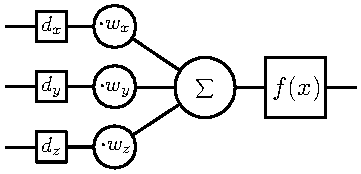
\includegraphics[width=0.85\textwidth]{SpikeBasedModel}
  \captionsetup{justification=centering, skip=5pt}
  \caption[Spiking Model]{Spiking Model}
  \label{fig:Spiking Model}
\end{subfigure}%
\begin{subfigure}{.4\textwidth}
  \centering
  \includegraphics[width=0.7\textwidth]{RatebasedModel}
  \captionsetup{justification=centering, skip=5pt}
  \caption{Rate-Based Model}
  \label{fig:Rate Based Model}
\end{subfigure}
\begin{subfigure}{.9\textwidth}
  \centering
  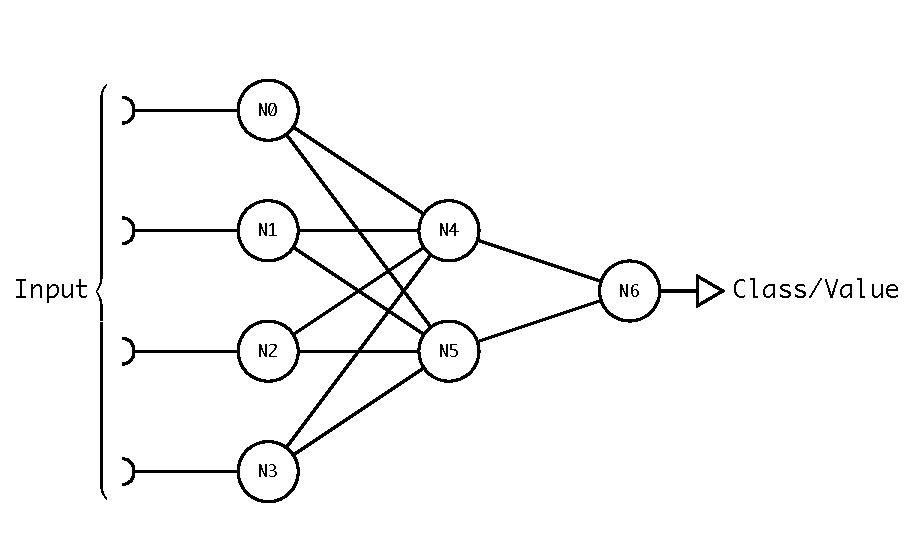
\includegraphics[width=0.7\textwidth]{SimpleNetwork}
  \captionsetup{justification=centering, skip=5pt}
  \caption{Network of Artificial Neurons}
  \label{fig:Network of ANs}
\end{subfigure}
\captionsetup{justification=centering, skip=6pt}
\caption[Artificial Neural Network]{Artificial Neurons and Network}
\label{fig:Artificial Neural Network}
\end{figure}

\begin{figure}
\centering
\begin{subfigure}{.3\textwidth}
  \begin{tikzpicture}[scale=0.5]
    \begin{axis}[
        title={Sigmoid},
        %grid = major,
        xmin=-6,xmax=6,
        ymin=0,ymax=1,
        legend style={draw=none, fill=white},      
        legend pos= outer north east
        ]
        \addplot[myBlueThickStyle] expression[domain=-6:6,samples=100]{1/(1+e^(-x))} 
                    node at (axis cs:3,0.7){}; 
        \legend{{\large $f(x)=\frac{1}{1+e^{-t}}$}}
    \end{axis}
  \end{tikzpicture}
  \captionsetup{justification=centering, skip=5pt}
  \caption{Sigmoid}
  \label{fig:Sigmoid}
\end{subfigure}%
\begin{subfigure}{.3\textwidth}
  \begin{tikzpicture}[scale=0.5]
    \begin{axis}[
        title={ReLu},
        xmin=-1,xmax=1,
        ymin=0,ymax=1,
        legend style={draw=none, fill=white},      
        legend pos= outer north east
        ]
        \addplot[myBlueThickStyle] expression[domain=0:1,samples=100]{x} node at (axis cs:0.6,0.15){}; 
         \addplot[myBlueThickStyle] expression[domain=-1:0,samples=100]{0};       
         % had to change , to f&%$$#$g \text{,} on max.ece.ncsu.edu, what BS
         \legend  {{ $f(x)= \begin{cases} 0\text{,}      &\text{if $x < 0$;}\\   x\text{,}       &\text{otherwise.}  \end{cases}$}}  
    \end{axis}
  \end{tikzpicture}
  \captionsetup{justification=centering, skip=5pt}
  \caption{Relu}
  \label{fig:Relu}
\end{subfigure}
\captionsetup{justification=centering, skip=5pt}
\caption{Example Rated-Based Model Activation functions}
\label{fig:Example Rated-Based Model Activation functions}
\end{figure}

\begin{figure}
\centering
\captionsetup{justification=centering}
\vspace{0.5cm}
\begin{subfigure}{.9\textwidth}
  \centering
  \begin{equation}
    \begin{split}
    &v' = 0.04v^2+5v + 140 - u - I\\
    &u' = a(bv-u)  \\
    &\text{if } v\ge  \SI{30}{\mV}, \text{ then } 
    \begin{cases}
        v \leftarrow c\\           
        u \leftarrow u+d\\           
    \end{cases} \nonumber
    \end{split}
  \end{equation}
  \caption{Izhikevich Model\cite{Iz2005}}
  \label{fig:Izhikevich Model}
  \end{subfigure}
\begin{subfigure}{.7\textwidth}
  \centering
  \mbox{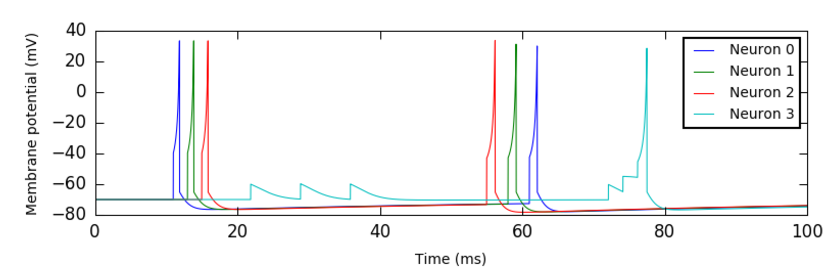
\includegraphics[width=4.0in]{SpikingExample.pdf}}
  \captionsetup{justification=centering, skip=3pt}
  \caption{Izhikevich Model Simulation \cite{Iz2005}\cite{carnevale2006neuron}}
  \label{fig:spiking example}
\end{subfigure}
\caption{Example Spiking Activation Function Model}
\label{fig:Example Spiking Model}
\end{figure}

To emulate complex behavior, the artifical neurons are connected in networks, typically with layers of sub-networks which are in affect separated by the non-linear activation function.
Examples of both rate-based and spiking artificial neural networks can be seen in \fref{fig:Rate-based Model Network} and \fref{fig:Spiking Model Network} respectively.
Typically neural networks process in a feed-forward fashion. Considering \fref{fig:Artificial Neural Network}, this means the input arrives on the left, the inputs propagate to neurons N0 through N3. WHen N0 through N3 are processed, their values propagate forward to neurons N4 and N5 etc.. SOmetime \ac{ann}s also include recursion where for example neurons N0 through N4 are not only influenced
by the input, but also by themselves. Many \ac{ann}s operate only in feed-forward fashion but some popular \ac{ann}s, such as Long short-term memory (LSTM), employ recursion.

Another popular \ac{ann} known as Deep Neural Networks (\ac{dnn}) have proved very popular over the last few years. They get good press in applications such as image recognition and speech recognition. 
Deep Neural Networks are often formed from tens of layers of \ac{an}s with each layer containing many \ac{an}s. \ac{dnn}s are also processed in a feed-forward manner with one layer being the inputs to the next layer. 
As mentioned \cite{krizhevsky2012imagenet}, these useful \ac{dnn}s often require hundreds of thousands of \ac{an}s and within the network, each \ac{an} can have hundreds, even thousands of feeder or pre-synaptic \ac{an}s.
There have been implementations that use different number formats from double precision floating point to eight bit integers, but in all cases these useful \ac{ann}s require a significant amount of memory to store the connection weights (parameters).


\begin{figure}[!t]
  % the [] contains position info e.g. [!t] means here
  \centering
  \captionsetup{justification=centering}
  \captionsetup{width=.9\linewidth}
  \begin{subfigure}{.9\textwidth}
    \centerline{
    \mbox{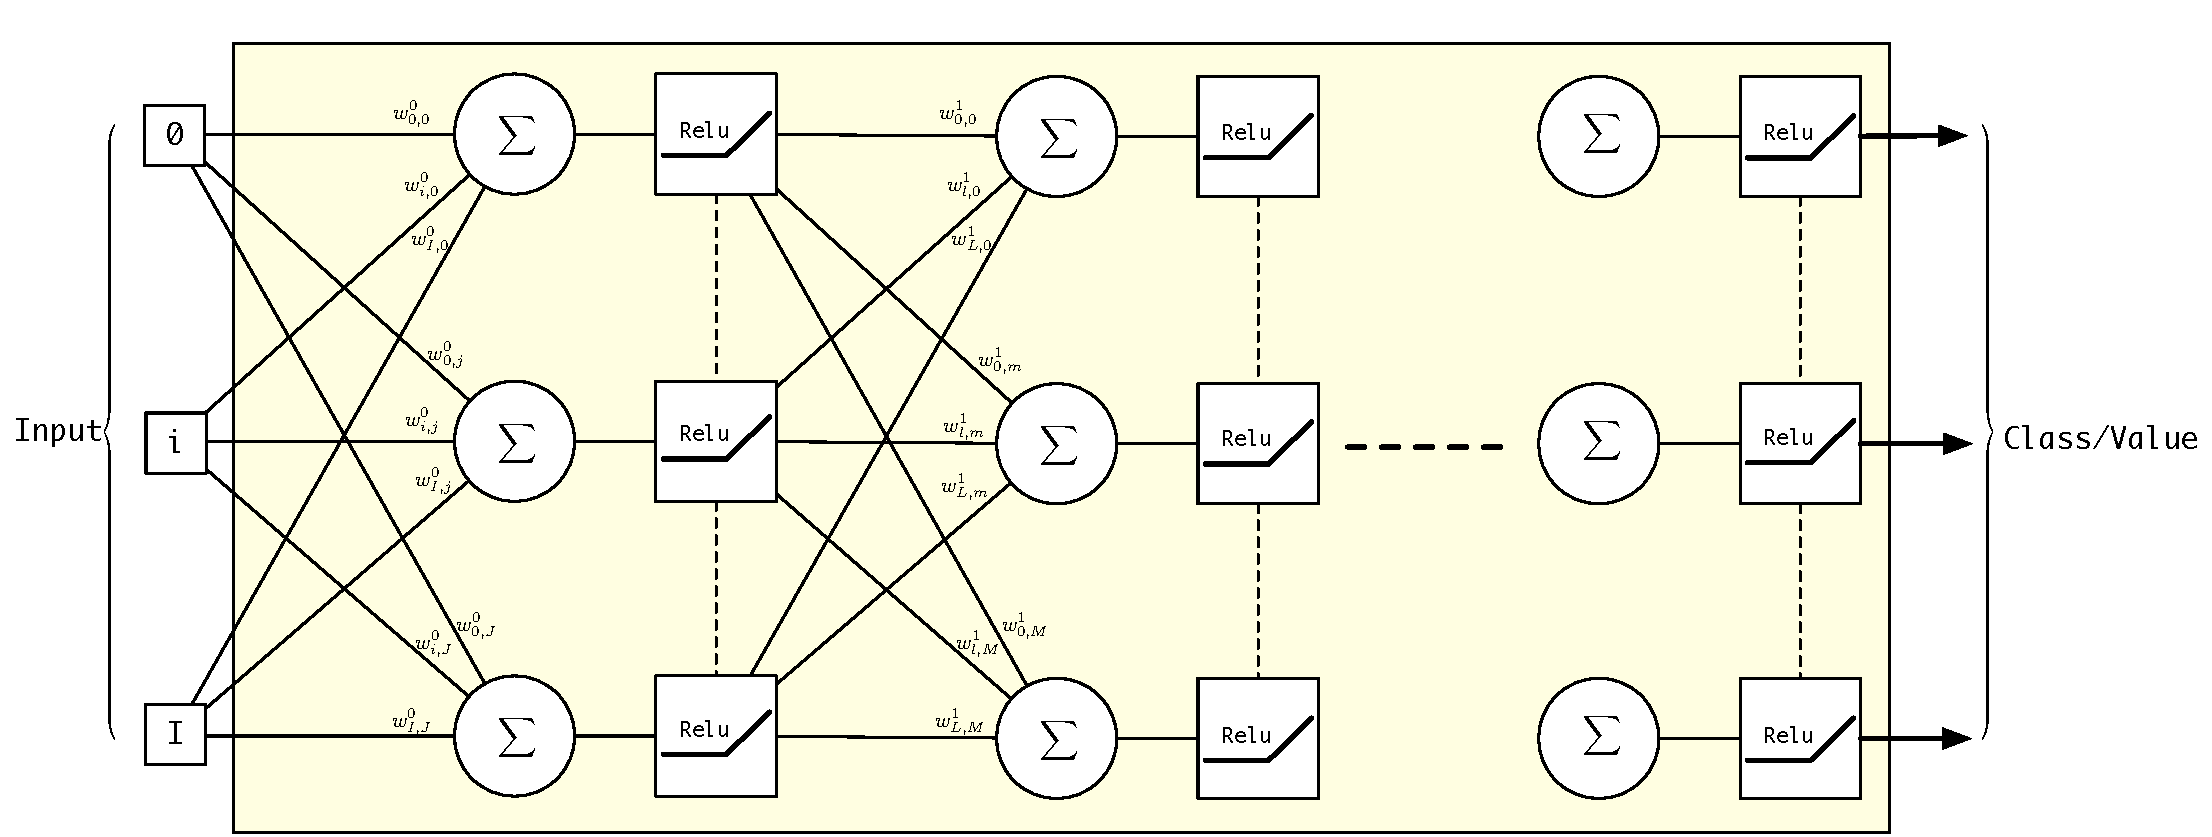
\includegraphics[width=0.85\textwidth]{RateBasedNeuralNetwork.pdf}}
    }
    \caption{Rate-based Model Artificial Neural Network (with ReLu activation function)}
    \label{fig:Rate-based Model Network}
  \end{subfigure}
  
  \begin{subfigure}{.9\textwidth}
    \centerline{
    \mbox{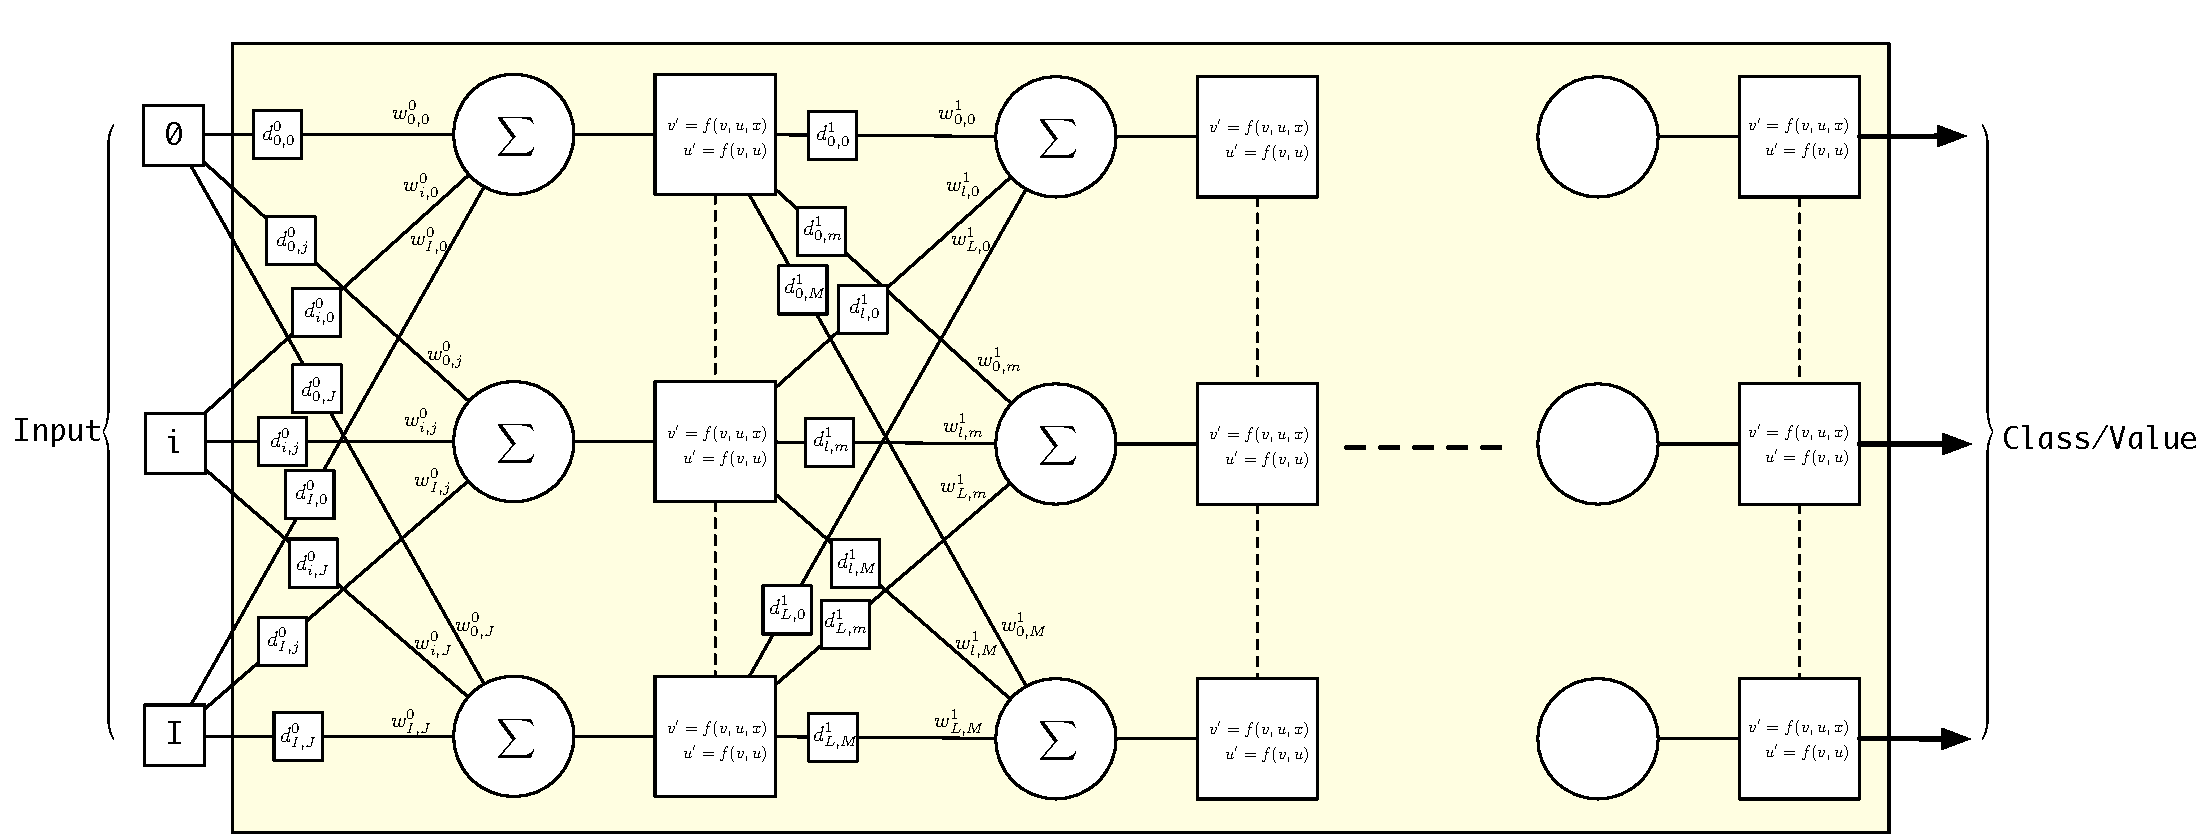
\includegraphics[width=0.85\textwidth]{SpikingNeuralNetwork.pdf}}
    }
    \caption{Spiking-based Model Artificial Neural Network}
    \label{fig:Spiking Model Network}
  \end{subfigure}
  \caption{Layered Artificial Neural Networks}
  \label{fig:Layered Artificial Neural Networks}
\end{figure}

Although the spiking neural network more closely models the behavior of real neurons, over the last 20 years there 
have been breakthroughs in the configuring of rate-based models especially with the introduction of the back-propagation
algorithm and stochastic gradient descent. Along with the abundance of data now available in the form of voice, images etc. to "teach" these networks
using back-propagation, most of the effective applications of artificial neural networks have employed these rate-based models.

\iffalse
Our research will focus on these rate-based models which we will now refer to as \ac{ann}s.
\fi

This work does not address the training of these rate-based \acp{ann}, the training is mostly performed offline. This work is addressing the inference of \acp{ann}.
During inference, the most computationally intensive operation is the multiply accumulate associated with the \ac{an} activation, which can involve hundreds or thousands of multiply-accumulates.
The \ac{an} activation calculation for the rate-based \ac{an} in figure \ref{fig:Rate Based Model} is shown in equation \eqref{eq:activation function}.

\begin{alignat}{2} 
\label{eq:activation function}
\text{\ac{an} Activation }\hspace{4mm} A & = f\bigg(\sum_{n=0}^{C_n}W_n \cdot A_n\bigg)  \\
              &\mathbf{C_p} \text{ is the number of pre-synaptic connections} \notag\\
              &\mathbf{W_p} \text{ is the weight of a connection} \notag\\
              &\mathbf{A_p} \text{ is the activation value of the pre-synaptic neuron} \notag \\
\text{and }   &f(x) \text{ is the activation function such as ReLu } \notag 
\end{alignat}

\section[ANN Layers]{ANN Layers}
\label{sec:ANN Layers}

In figures \ref{fig:Network of ANs} and \ref{fig:Rate-based Model Network}, the \ac{ann} is shown to be constructed using layers of \acp{an}. It has long been known that a single layer of \acp{an} can be used linearly partition an n-dimensional input, as shown in figure \ref{fig:linear discrimination}.
However, if a more complex partition is required, this cannot be achieved using a single layer of \acp{an}. A higher order classification, as shown in figure \ref{fig:linear discrimination} can only be achieved using multiple layers of \acp{an}. 
In addition, to ensure the multiple layers cannot be mathematically collapsed into a single layer, the activation function $f(x)$, as shown in figure \ref{fig:Rate Based Model} must be a non-linear function.



\begin{figure}[h]
\centering
  \begin{subfigure}{.4\textwidth}
    \centering
    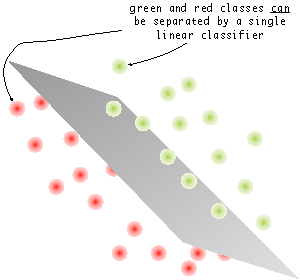
\includegraphics[width=0.85\textwidth]{linearDiscrimination}
    \captionsetup{width=.8\textwidth, justification=centering, skip=20pt}
    \caption{Linear Classification using a single layer}
    \label{fig:linear discrimination}
  \end{subfigure}%
  \begin{subfigure}{.4\textwidth}
    \centering
    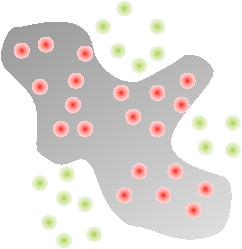
\includegraphics[width=0.7\textwidth]{complexDiscrimination}
    \captionsetup{width=.8\textwidth, justification=centering, skip=10pt}
    \caption{Complex Classification requires multiple layers}
    \label{fig:complex discrimination}
  \end{subfigure}
\captionsetup{justification=centering, skip=10pt}
\caption{Classification using \acp{ann} layers}
\label{fig:Discrimination}
\end{figure}


\subsection{Deep Neural Networks}
\label{sec:Deep Neural Networks}

As mentioned, a single layer of neurons can be used as a linear classifier as long as the classes can be separated using a linear function.
Even some simple cases cannot be linearly separated, an example often used is an exclusive-OR gate.

Even with a layered \ac{ann}, the final output comes from a single layer. To allow this final layer to linearly separate classes, the original input needs to be transformed into a space where the classes can be linearly separated.
\acf{dnn} are \acp{ann} that incorporate many layers of \acp{an}, often which are often up to tens of layers deep.
The additional layers are incorporated to translate the space of the input so the various classes being identified can be separated using linear classifiers in the later layers.

Recently, an example of a \ac{dnn} known as a \acf{cnn} demonstrated high levels of efficacy when used to classify objects in images \cite{krizhevsky2012imagenet}.
These \acp{cnn} use the early layers to identify low-level features and later layers are used combine these features into yet more higher-level features.
Finally, the combination of high-level features are used to identify the required classes.
This layering is shown in \fref{fig:Deep network showing feature layers}.
\begin{figure}[h]
\centering
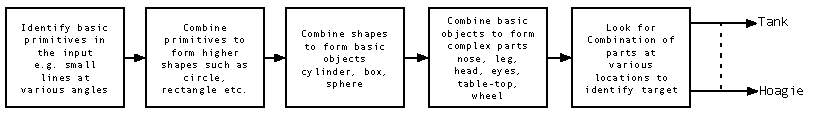
\includegraphics[width=0.95\textwidth]{deepNetworkBlockDiagram}
\captionsetup{justification=centering, skip=5pt}
\caption{Deep network showing feature layers}
\label{fig:Deep network showing feature layers}
\end{figure}

In figure \ref{fig:Deep network showing feature layers}, the final layer is often a fully connected linear classifier with the output representing the probability of a particular class being present in the image.
In practice, these \acp{dnn} can be used as classifiers or as function approximators.

\iffalse
In practice, useful deep neural networks are very large and often exceed the capacity of single GPUs. Therefore,  there is opportunity for a solution that provides
real-time acceleration and storage of of these systems.
\fi


\subsection{Feature Layers}
\label{sec:Feature Layers}

For the most part, different \acp{ann} are characterized by how the \acp{an} are interconnected and the activation function employed.

The typical \ac{dnn} layers are processed in a feed-forward fashion where the pre-synaptic \acp{an} are formed from \acp{an} in the previous layer.
There are some types of \ac{dnn} which also include recursive connections where the the pre-synaptic \acp{an} include \acp{an} from the current layer.
A popular recursive \ac{dnn} is \acf{lstm}. Although this work does not preclude supporting \ac{lstm} in the future, the focus of this work is on the feed-forward type \ac{dnn}.

As described in \ref{sec:Deep Neural Networks}, a \ac{dnn} layer transforms the previous layer with each higher layer providing a coarser grained transformation. This is best seen in image recognition application were the early layers identify low level shapes or features, such as angled lines. 
The following layers are used to identify higher order shapes such as circles, blocks etc. 
Although the features detected during the image recognition application are somewhat intuitive, it is believed that in less intuitive applications the \ac{dnn} performs a similar fine to coarse feature extraction.

The connections between layers can be locally-connected or fully-connected. 
With locally-connected layers as shown in figure \ref{fig:Locally Connected Layer to Layer Connection Types}, a layers pre-synaptic \acp{an} are formed from regions of the previous layer.
With fully-connected layers as shown in figure \ref{fig:Fully Connected Layer to Layer Connection Types}, a layers pre-synaptic \acp{an} are formed from all \acp{an} in the previous layer.
In many cases, a \ac{dnn} is constructed with lower layers being locally-connected and higher layers being fully connected.

\begin{figure}[h]
  \centering

  \begin{subfigure}{1.0\textwidth}
    \centering
    \begin{subfigure}{.5\textwidth}
      \centering
      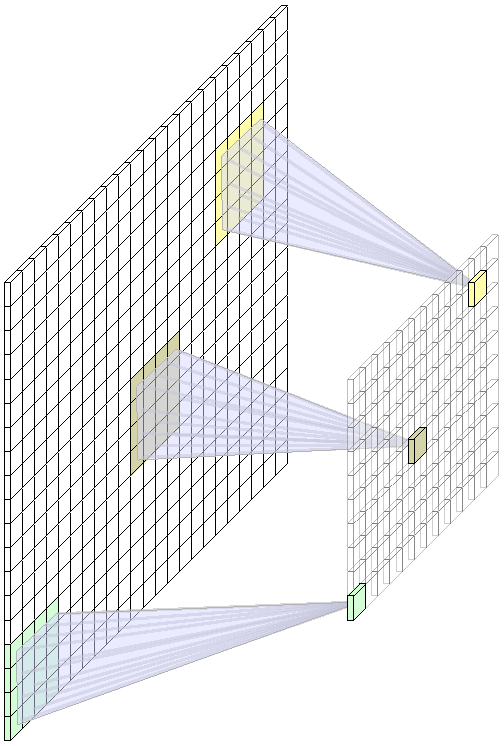
\includegraphics[width=0.50\textwidth]{localArrayToArrayConnections}
      \captionsetup{width=.8\textwidth, justification=centering, skip=10pt}
      \caption{Local Array to Array}
      \label{fig:Local Array to Array}
    \end{subfigure}%
    \begin{subfigure}{.5\textwidth}
      \centering
      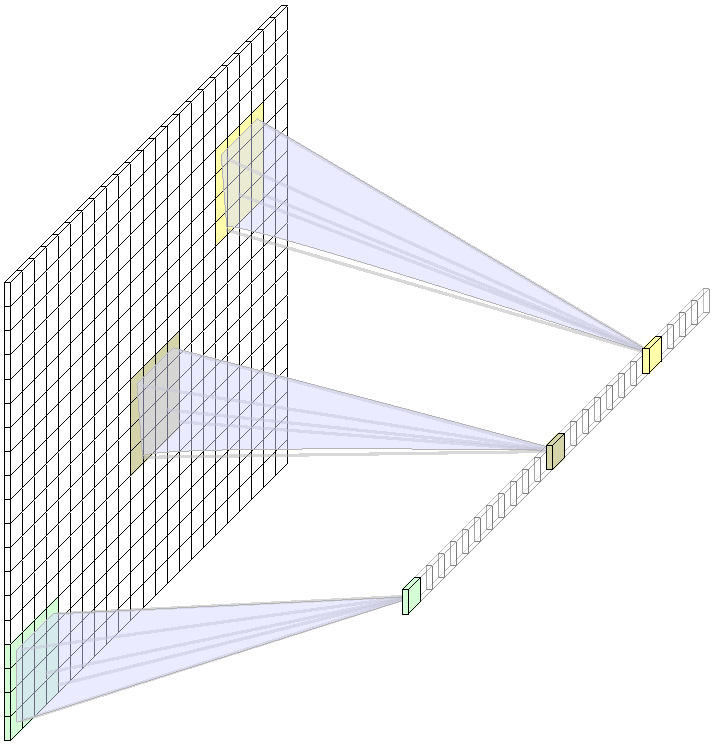
\includegraphics[width=0.70\textwidth]{localArrayToLinearConnections}
      \captionsetup{width=.8\textwidth, justification=centering, skip=10pt}
      \caption{Local Array to Linear}
      \label{fig:Local Array to Linear}
    \end{subfigure}
  \end{subfigure}

  \bigskip

  \begin{subfigure}{1.0\textwidth}
    \centering
    \begin{subfigure}{.5\textwidth}
      \centering
      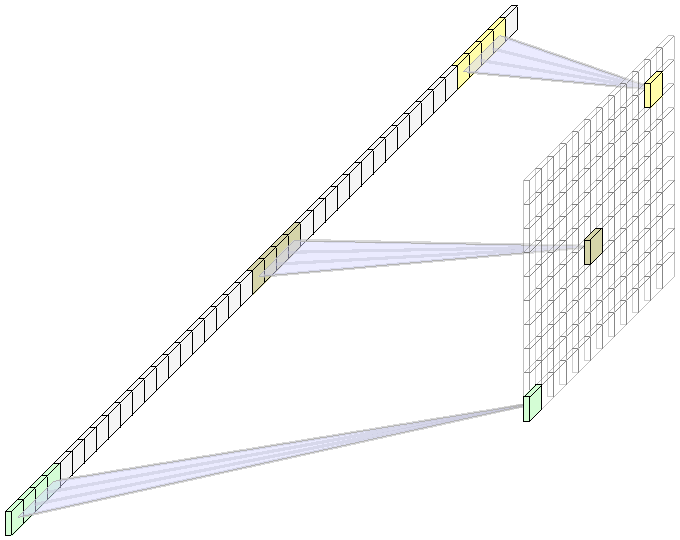
\includegraphics[width=0.60\textwidth]{localLinearToArrayConnections}
      \captionsetup{width=.8\textwidth, justification=centering, skip=10pt}
      \caption{Local Linear to Array}
      \label{fig:Local Linear to Array}
    \end{subfigure}%
    \begin{subfigure}{.5\textwidth}
      \centering
      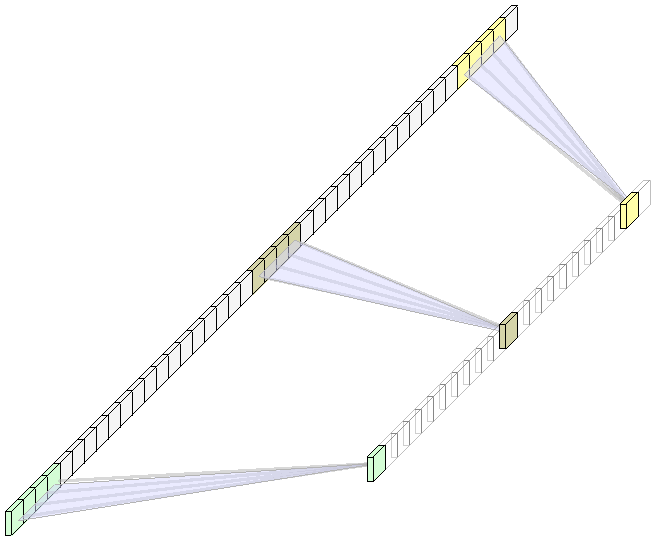
\includegraphics[width=0.60\textwidth]{localLinearToLinearConnections}
      \captionsetup{width=.8\textwidth, justification=centering, skip=10pt}
      \caption{Local Linear to Linear}
      \label{fig:Local Linear to Linear}
    \end{subfigure}
  \end{subfigure}

\captionsetup{justification=centering, skip=10pt}
\caption{Locally Connected Layer to Layer Connection Types}
\label{fig:Locally Connected Layer to Layer Connection Types}
\end{figure}

\begin{figure}[h]
  \centering
  \begin{subfigure}{1.0\textwidth}
    \centering
    \begin{subfigure}{.5\textwidth}
      \centering
      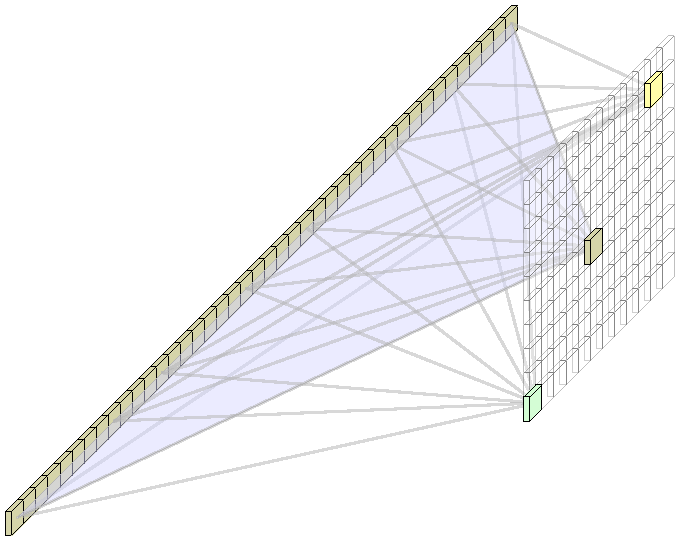
\includegraphics[width=0.60\textwidth]{fullLinearToArrayConnections}
      \captionsetup{width=.8\textwidth, justification=centering, skip=10pt}
      \caption{Full Linear to Array}
      \label{fig:Full Linear to Array}
    \end{subfigure}%
    \begin{subfigure}{.5\textwidth}
      \centering
      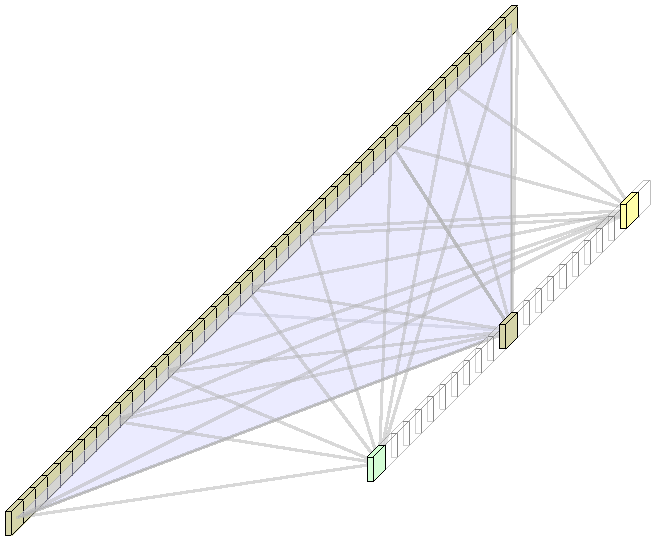
\includegraphics[width=0.60\textwidth]{fullLinearToLinearConnections}
      \captionsetup{width=.8\textwidth, justification=centering, skip=10pt}
      \caption{Full Linear to Linear}
      \label{fig:Full Linear to Linear}
    \end{subfigure}
  \end{subfigure}

  \bigskip

  \begin{subfigure}{1.0\textwidth}
    \centering
    \begin{subfigure}{.5\textwidth}
      \centering
      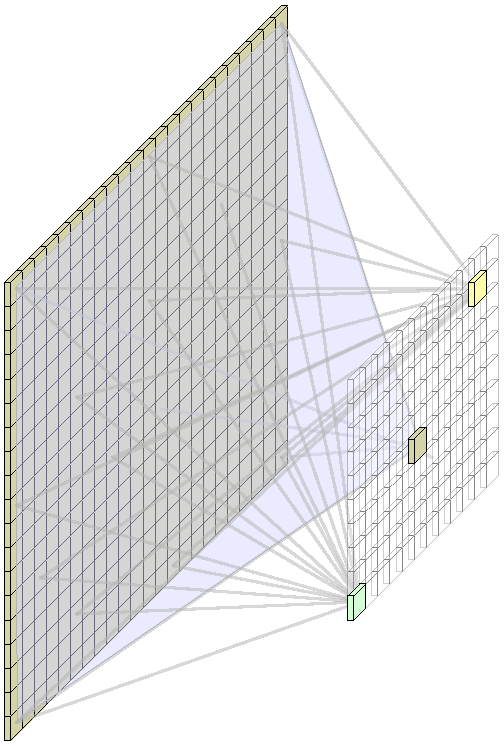
\includegraphics[width=0.50\textwidth]{fullArrayToArrayConnections}
      \captionsetup{width=.8\textwidth, justification=centering, skip=10pt}
      \caption{Full Array to Array}
      \label{fig:Full Array to Array}
    \end{subfigure}%
    \begin{subfigure}{.5\textwidth}
      \centering
      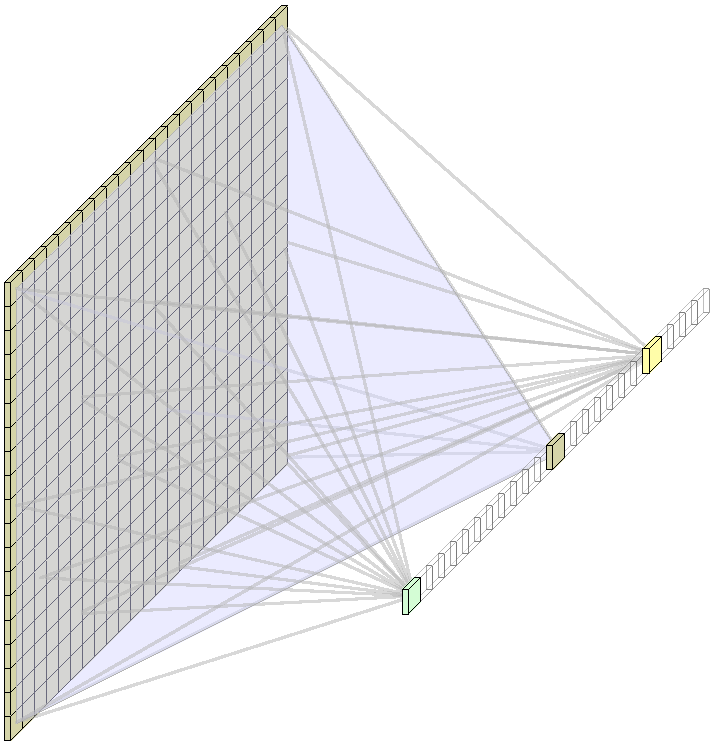
\includegraphics[width=0.7\textwidth]{fullArrayToLinearConnections}
      \captionsetup{width=.8\textwidth, justification=centering, skip=10pt}
      \caption{Full Array to Linear}
      \label{fig:Full Array to Linear}
    \end{subfigure}
  \end{subfigure}

\captionsetup{justification=centering, skip=10pt}
\caption{Fully Connected Layer to Layer Connection Types}
\label{fig:Fully Connected Layer to Layer Connection Types}
\end{figure}

\iffalse With locally-connected layers, the connection weights of the pre-synaptic \acp{an} are often formed from wanting to identify particular features. \fi
In early uses of locally-connected \acp{ann}, the first layers weights were often hand-generated, an example being Gabor filters. 
With automatically trained \acp{ann}, the feature detectors at each layer are often created during training.
Some contrived examples of locally-connected feature detectors are shown in figure \ref{fig:Features and locally-connected filters (kernels)}.
\begin{figure}[h]
\centering
  %\begin{subfigure}{.7\textwidth}
    %\centering
    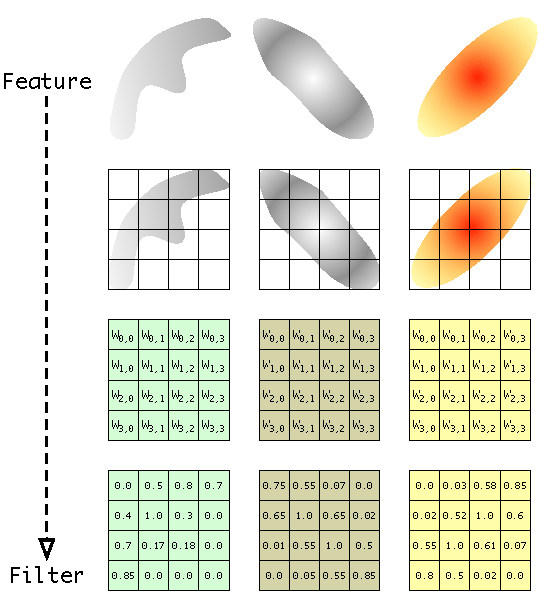
\includegraphics[width=0.55\textwidth]{locallyConnectedFeatures}
    \captionsetup{justification=centering, skip=5pt}
    \caption{Features and locally-connected filters (kernels)}
    \label{fig:Features and locally-connected filters (kernels)}
  %\end{subfigure}%
\end{figure}

The pre-synaptic \acp{an} of a locally-connected \ac{an} are formed from particular \ac{roi} of the previous layer using the weights from a feature filter. 
Another locally-connected \ac{an} may use the same \ac{roi} but employs a different filter.
In practice, for a particular \ac{roi}, a number of feature filters are employed resulting in a number of \acp{an} being associated with the same \ac{roi} in the previous layer. 
To reiterate, these feature filters all operate on the same \ac{roi}.
A different \ac{roi} will result in another group of \acp{an} all using their own feature filters.
The resulting locally-connected layer becomes a \ac{3d} layer with its X-Y coordinates representing a reference to a particular \ac{roi} and the Z-dimension representing the various filters applied to that \ac{roi}.
A example \ac{3d} locally-connected layer can be seen in figure \ref{fig:3D layers of Features}.

\iffalse
A good example of the feature filters is image recognition \acp{ann}. The lower level features generated during automatic training are often intuitive and the filters are constructed to detect small features such as lines at various angles, different curves etc..
In the general \ac{dnn} case, the trained feature detectors may not be as intuitive.
\fi
  %\bigskip

\begin{figure}[h]
\centering
  %\begin{subfigure}{.7\textwidth}
    %\centering
    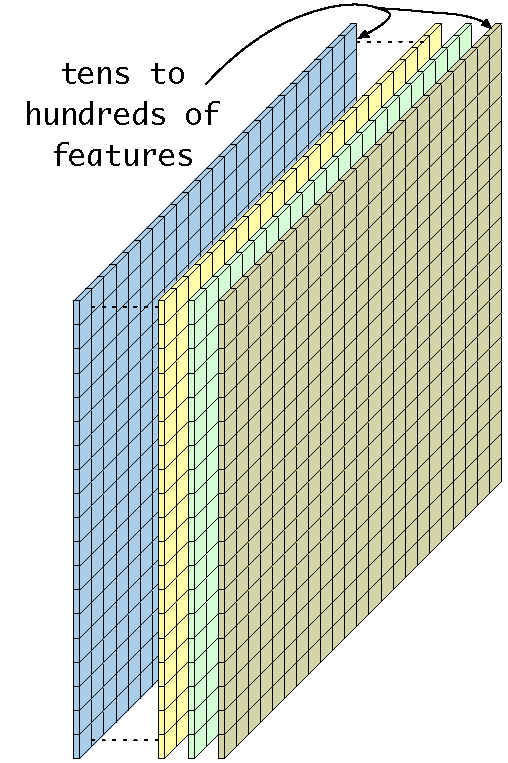
\includegraphics[width=0.35\textwidth]{layer3DFeatures}
    \captionsetup{justification=centering, skip=5pt}
    \caption{Single Layer constructed from 3D layers of Features}
    \label{fig:3D layers of Features}
  %\end{subfigure}
%\captionsetup{justification=centering, skip=10pt}
%\caption{Layer Feature Planes}
\label{fig:Layer Features}
\end{figure}

%%\begin{figure}[h]
%%\centering
%%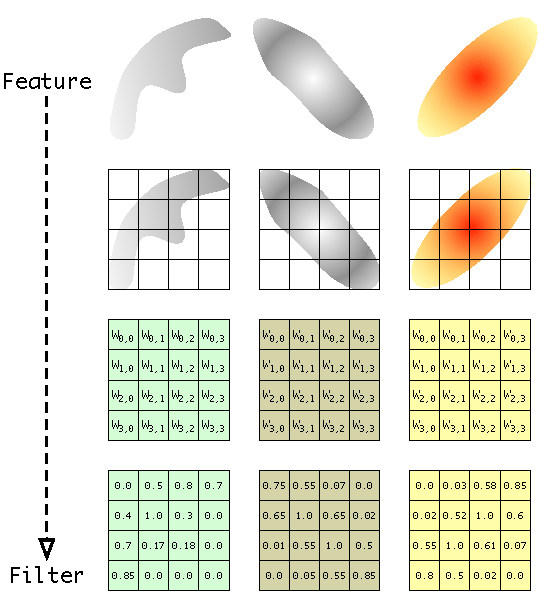
\includegraphics[width=0.55\textwidth]{locallyConnectedFeatures}
%%\captionsetup{justification=centering, skip=5pt}
%%\caption{Features and locally-connected filters (kernels)}
%%\label{fig:Features and locally-connected filters (kernels)}
%%\end{figure}
%%
%%\begin{figure}[h]
%%\centering
%%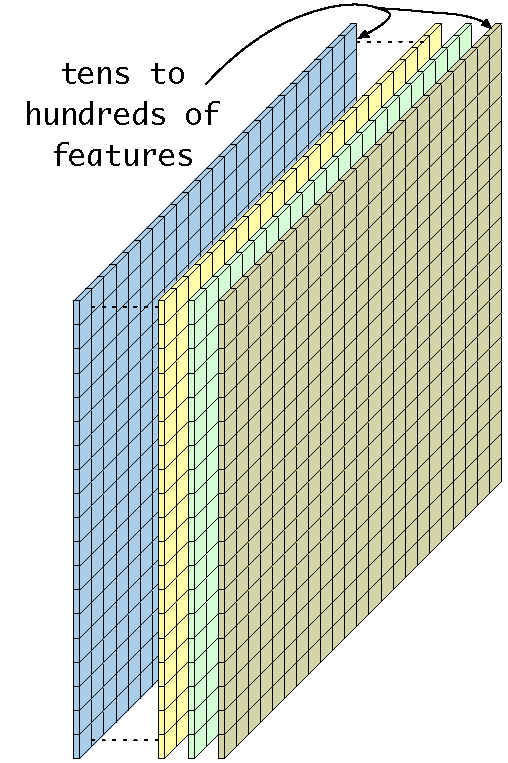
\includegraphics[width=0.55\textwidth]{layer3DFeatures}
%%\captionsetup{justification=centering, skip=5pt}
%%\caption{Features form 3D layers}
%%\label{fig:Features form 3D layers}
%%\end{figure}

So these locally-connected layers have multiple filters applied to the same \ac{roi} and the next layer becomes a \ac{3d} array with the Z-axis representing the features. 
The number of feature filters applied at each layer can be tens to hundreds of filters.
The filters employed in a layer following one of these \ac{3d} locally-connected layers are themselves 3D. With tens to hundreads of features in the previous layer the number of weights associated with each filter is usually hundreds to thousands of weights. 

The feature filters employed in the locally-connected layers can be unique to the regions of the previous layer or the same filters can be employed across the entire previous layer.
In the case of employing the same filters across the entire input layer the \ac{ann} is known as a \acf{cnn}. The \acp{cnn} are examples of \acp{ann} which can take advantage of reuse described in chapter \ref{sec:chap-one}. 
These \acp{cnn} can store the filter parameters in local \ac{sram} and construct an entire feature plane. These \acp{cnn} are considered a subset of the generic case of \ac{dnn}.
This work considers the more general \ac{dnn} case and supports acceleration of generic \acp{dnn} which includes \acp{cnn}.

An example of a \ac{dnn} can be seen in figure \ref{fig:DNN showing layer order} with the layer configurations shown in table \ref{tab:Layer Configuration}. A \ac{cnn} similar to this has demonstrated high levels of efficacy in image recognition applications.
{\textbf{\textcolor{black}{Therefore, this work will use the parameters from the table shown in figure \ref{tab:Layer Configuration} as a template for estimating the storage and processing requirements and the range of pre-synaptic fanins.}}}

%%
\iffalse
\begin{table}[ht]
\centering
\begin{tabular}{|c|c|c|c|c|c|c|c|}\cline{3-8}
\multicolumn{2}{c|}{\multirow{2}{*}{}}&\multicolumn{3}{c|}{Singular}&\multicolumn{3}{c|}{Plural}\\\cline{3-8}
\multicolumn{2}{c|}{}&Neuter&Masculine&Feminine&Masculine&Feminine&Neuter\\\hline
\multicolumn{1}{|c|}{\multirow{2}{*}{I}}&Inclusive&\multicolumn{3}{|c|}{\multirow{2}{*}{O}}&\multicolumn{3}{c|}{X}\\\cline{2-2}\cline{6-8}
&Exclusive&\multicolumn{3}{c|}{}&\multicolumn{3}{c|}{X}\\\hline
\multirow{2}{*}{II}&Informal&\multicolumn{3}{|c|}{X}&\multicolumn{3}{c|}{X}\\\cline{2-8}
&Formal&\multicolumn{6}{|c|}{X}\\\hline
\multirow{2}{*}{III}&Informal&\multicolumn{1}{c|}{\multirow{2}{*}{O}}&X&X&\multicolumn{2}{|c|}{X}&\multicolumn{1}{c|}{\multirow{2}{*}{O}}\\\cline{2-2}\cline{4-7}
&Formal&&\multicolumn{4}{|c|}{X}&\\\hline

\end{tabular}
\end{table}
\fi

\begin{sidewaysfigure}[h]
  %\begin{adjustbox}{angle=0, width=1.0\textwidth}
    \centering
    \captionsetup{justification=centering}
    \begin{subtable}{.9\textwidth}
      %\captionsetup{justification=centering, skip=-5pt}
      \centering
      %\begin{center}
       % [lr] ~ left align col 0 and right align col 1
       % e.g. 4 columns could be lccr
      \begin{adjustbox}{width=1\textwidth}
        \begin{tabular}{|r|c|c|c|c|c|c|c|c|c|c|c|c|c}\cline{3-13}
          %\toprule
           \multicolumn{2}{c|}  {\multirow{2}{*}{}}    & \multicolumn{11}{c|}{Layers}    \\\cline{3-13}
           \multicolumn{2}{c|}{}                       &  1 & 2 & 3 & 4 & 5 & 6 & 7 & 8 & 9 & 10 & 11  \\\cline{3-13} \cline{1-13}
           \multicolumn{2}{|r|}{Type}                  &  Input          & Locally      & Pooling           & Locally             & Pooling             & Locally             & Locally             & Locally             &  Fully              &  Fully                 &  Fully         &                                    \\\cline{1-13}
           \multirow{3}{*}{Dimensions}               &X& \num{       256}& \num{     55}& \num{    27}      & \num{     27}       & \num{     13}       & \num{     13}       & \num{     13}       & \num{     13}       & \num{      4096}    & \num{     4096}        & \num{    1024} &                                    \\
                                                     &Y& \num{       256}& \num{     55}& \num{    27}      & \num{     27}       & \num{     13}       & \num{     13}       & \num{     13}       & \num{     13}       & \num{         1}    & \num{        1}        & \num{       1} &                                    \\
                                                     &Z& \num{         3}& \num{     96}& \num{    96}      & \num{    256}       & \num{    256}       & \num{    384}       & \num{    384}       & \num{    256}       & \num{         1}    & \num{        1}        & \num{       1} &                                    \\\cline{1-13}
           \multirow{3}{*}{Filter Dimensions}        &X&    na           & \num{     11}& \num{     2}      & \num{      5}       & \num{      2}       & \num{      3}       & \num{      3}       & \num{      3}       & \num{        13}    & \num{     4096}        & \num{    4096} &                                    \\
                                                     &Y&    na           & \num{     11}& \num{     2}      & \num{      5}       & \num{      2}       & \num{      3}       & \num{      3}       & \num{      3}       & \num{        13}    & \num{        1}        & \num{       1} &                                    \\
                                                     &Z&    na           & \num{      3}& \num{     1}      & \num{     96}       & \num{      1}       & \num{    256}       & \num{    384}       & \num{    384}       & \num{       256}    & \num{        1}        & \num{       1} &                                    \\\cline{1-14}
            \multicolumn{2}{|r|}{Stride           }    &    na           & \num{      4}& \num{     2}      & \num{      2}       & \num{      2}       & \num{      1}       & \num{      1}       & \num{      1}       &              na     &             na         &            na  & \multicolumn{1}{c|}{Aggregate    } \\\cline{14-14}
            \multicolumn{2}{|r|}{Pre-synaptic Fanin}   &    na           & \num{    363}& \num{     4}      & \num{   2400}       & \num{      4}       & \num{   2304}       & \num{   3456}       & \num{   3456}       & \num{     43264}    & \num{     4096}        & \num{    4096} & \multicolumn{1}{c|}{$\Bar{\num{   1650}}$} \\
            \multicolumn{2}{|r|}{Number of \ac{an}}    & \num{    196608}& \num{ 290400}& \num{ 69984}      & \num{ 186624}       & \num{  43264}       & \num{  64896}       & \num{  64896}       & \num{  43264}       & \num{      4096}    & \num{     4096}        & \num{    1024} & \multicolumn{1}{c|}{\num{ 969152}} \\
            \multicolumn{2}{|r|}{Number of Weights}    &    na           & \num{  34848}& na                & \num{ 614400}       & na                  & \num{ 884736}       & \num{ 1327104}      & \num{ 884736}       & \num{ 177209344}    & \num{ 16777216}        & \num{ 4194304} & \multicolumn{1}{c|}{\num{ 2.02e8}} \\\hline
        \end{tabular}
      \end{adjustbox}
      \captionsetup{justification=centering, skip=9pt}
      \vspace{0.5cm}
      \caption{Layer Configuration \cite{krizhevsky2012imagenet}}
      \label{tab:Layer Configuration}
      %  \end{center}
    \end{subtable}
  
    \bigskip

    %\begin{adjustbox}{width=1.0\textwidth}
      \begin{subfigure}{1\textwidth}
        \centering
        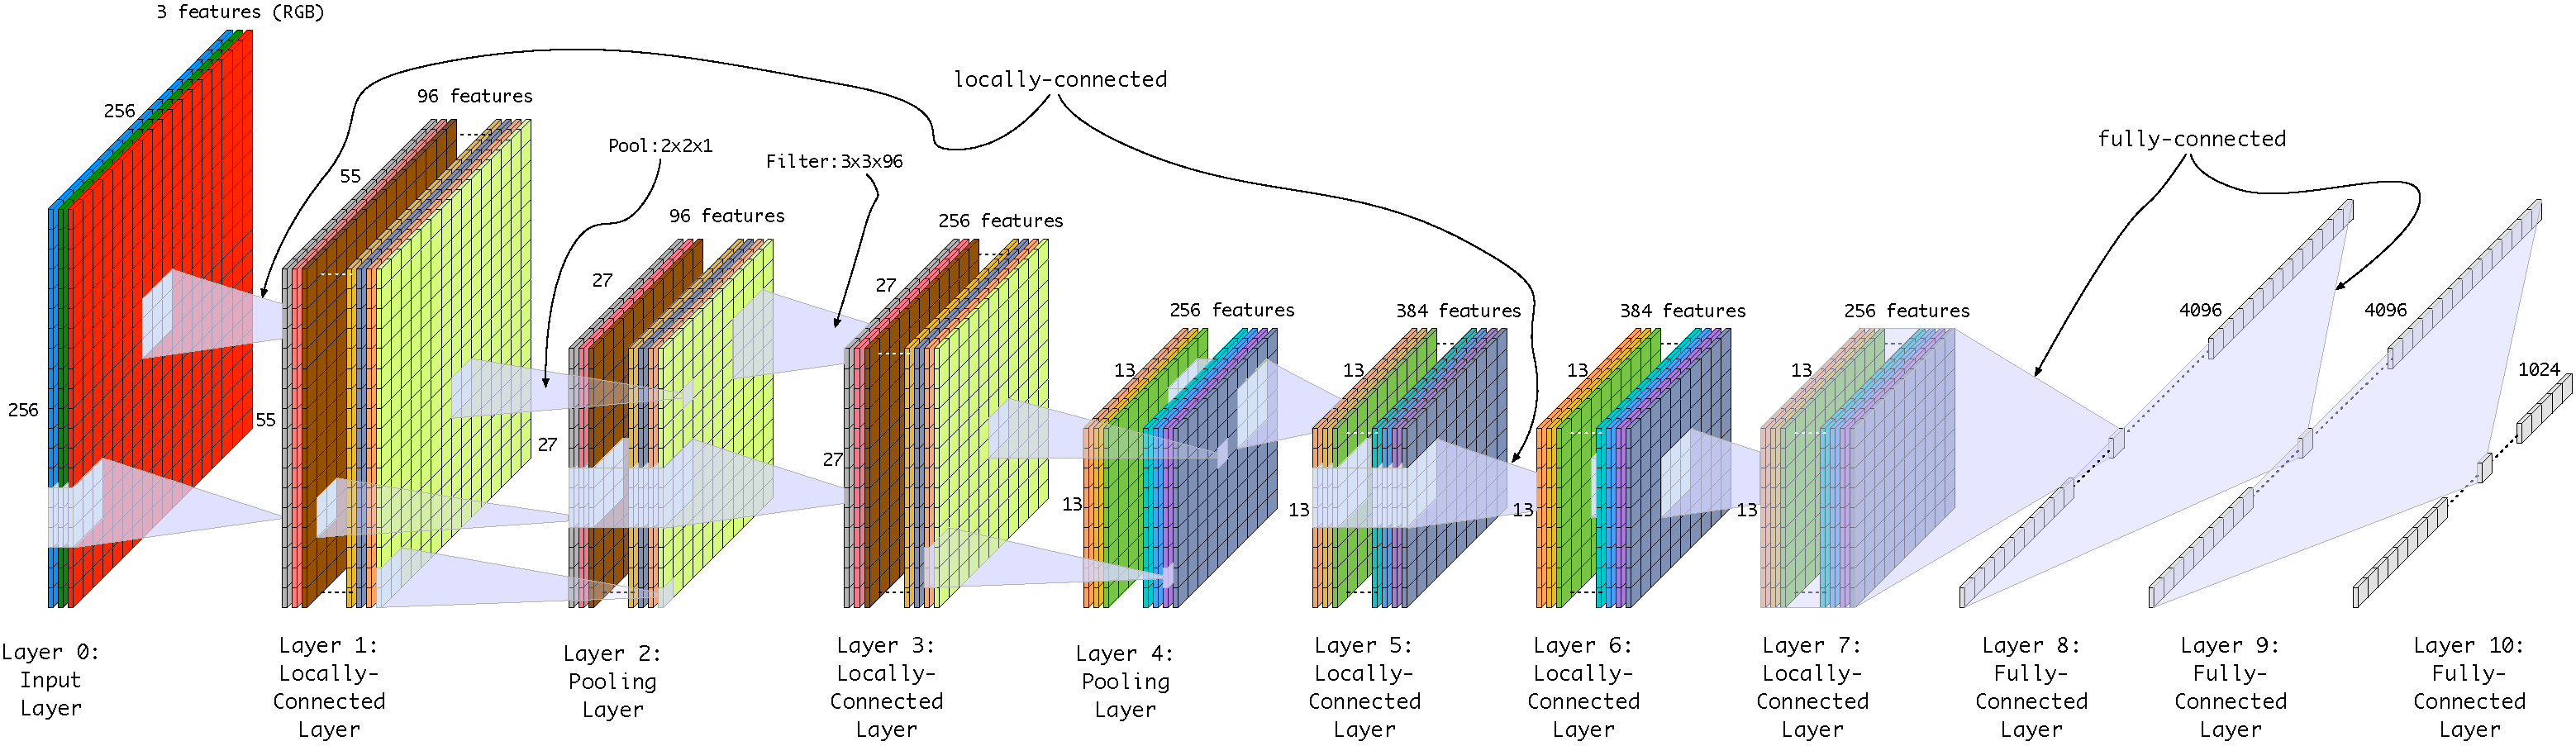
\includegraphics[width=1.0\textwidth]{fullDNN}
        \captionsetup{justification=centering, skip=15pt}
        \caption{DNN showing layer order \cite{krizhevsky2012imagenet}}
        \label{fig:DNN showing layer order}
      \end{subfigure}
    %\end{adjustbox}
  
  %\end{adjustbox}
  \caption{Baseline DNN \cite{krizhevsky2012imagenet}}
  \label{fig:Baseline DNN}
\end{sidewaysfigure}



\iffalse
\begin{sidewaysfigure}[h]
\centering
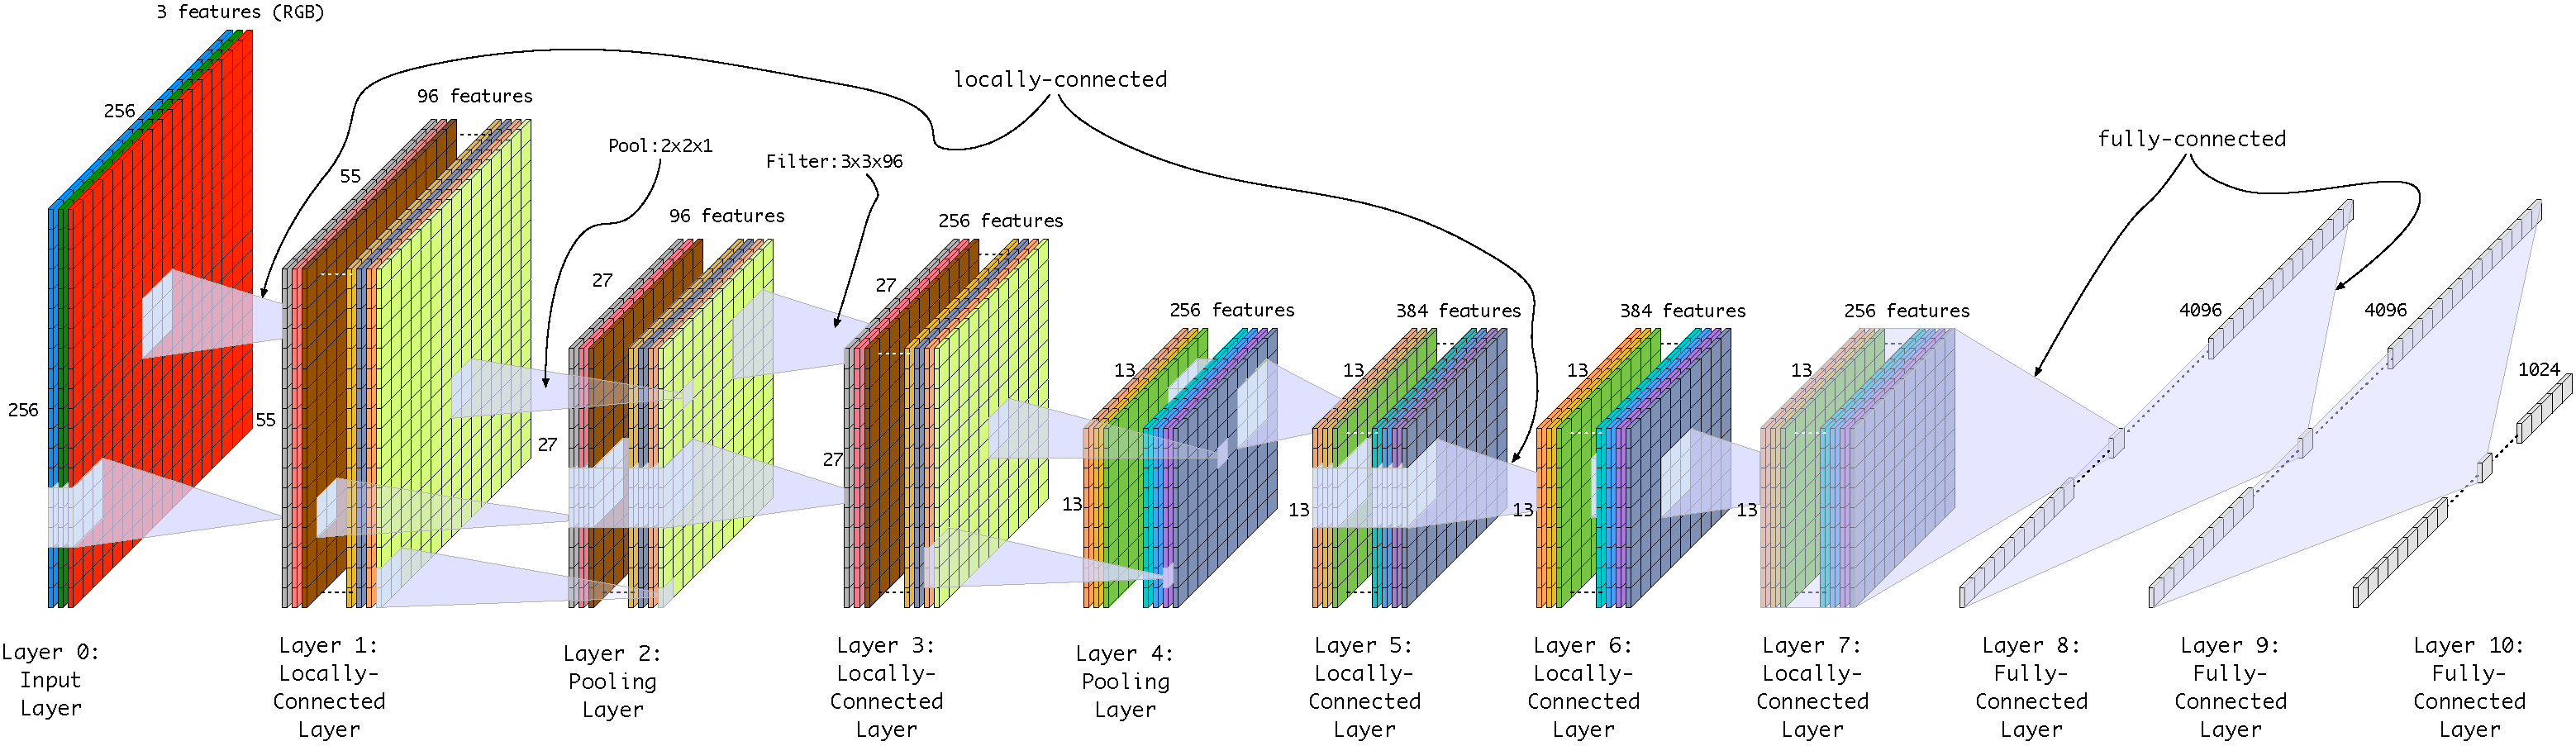
\includegraphics[width=1.0\textwidth]{fullDNN}
\captionsetup{justification=centering, skip=15pt}
\caption{DNN showing layer order \cite{krizhevsky2012imagenet}}
\label{fig:DNN showing layer order}
\end{sidewaysfigure}
\fi

To approach the capabilities observed in human behavior, such as object recognition \ac{ann}s have become very large. The example shown in figure \ref{fig:Baseline DNN}, which is based on the work from \cite{krizhevsky2012imagenet}, has hundreds of thousands of \acp{an} and hundreds of millions of connection weights (see table \ref{tab:Layer Configuration}).
These \acp{ann} utilize these hundreds of thousands of \acp{an} to implement what a human would consider a relatively straightforward task.
For example, a "useful" \ac{ann} similar to that described in \cite{krizhevsky2012imagenet} which was used to recognize up to 1000 different object classes, has a network size of approximately 650,000 \acp{an} and 630 million synaptic connections \cite{krizhevsky2012imagenetPreso}. 

The increased performance of \ac{ann}s over classical methods in image recognition and voice recognition might suggest that \ac{ann}s will out-perform operations performed in other applications.
\iffalse There is reason to believe that \acp{ann} will replace various functions in existing systems. \fi

If \ac{ann}s fulfill their potential, systems employing \ac{ann}s will utilize them for various functions, such as engine monitoring, anomaly detection, navigation etc. all within the same system.
Considering the various functions a complex customer facing or edge application system performs, it is likely that many real-world applications will employ multiple disparate instances of these useful sized \ac{ann}s.
Assuming these complex functions will require \ac{ann}s similar in size to figure \ref{fig:Baseline DNN} and \cite{krizhevsky2012imagenet}, these implementations will be processing multiple large \ac{ann}s at or near real-time.

\section[ANN Processing]{ANN Processing}
\label{sec:ANN Processing}

Considering the storage required for the input, the \ac{an} states and most significantly the weights for connections, the storage requirements results in gigabytes of memory.
When these \ac{ann}s are required to be solved in fractions of a second, the processing and memory bandwidth becomes prohibitive.

As a metric, this work assumes that any useful \ac{ann} will be similar to that shown in figure \ref{fig:Baseline DNN} which utilizes $>\num{900e3}$\acp{an} and $\approx\num{200e6}$ parameters. 
\iffalse
Given the bandwidth and storage requirements shown in table \ref{tab:Bandwidth and Storage Design Requirements}, the problem becomes \hyphenquote{american}{\textbf{\textcolor{black}{to provide deterministic at or near real-time performance within tolerable power and space constraints for edge systems employing inference on multiple disparate useful-sized neural networks.}}}
\fi
%\hlc[gray]{hello}
\iffalse
Considering that \ac{dram} is required to store the \ac{ann} parameters, why is it that much of the \ac{asic} and \ac{asip} \ac{ann} research employs \ac{sram} as an intermediate store? Well, in practice there are benefits if you can operate solely out of \ac{sram}.
Certainly good performance and potentially low power.
But use of \ac{sram} makes assumptions on the type of \acp{ann} that can be supported and the application in which the \ac{ann} is being deployed.
The primary requirement of the type of \ac{ann} and the deployed application to allow effective use of \ac{sram} is "reuse". Reuse means that once parameters are transferred and stored in \ac{sram}, these parameters can be reused such that the \ac{sram} isn't simply an intermediate memory but something akin to a cache.

In some \ac{ann}s there are reuse opportunities. A prime example is \acp{cnn}, where the connection weights are reused. In \acp{cnn}, a common filter is passed across an input to form the next layer. These filter "kernels" can be held in memory and the input is read from \ac{dram} thus reducing the \ac{dram} bandwidth.
Even with \ac{dnn}s where weights may not be reused, when implementing multiple \ac{dnn}s, there is opportunity to hold the input in memory.
If the system is being employed in cloud applications or in training, there is opportunity to reuse inputs whilst performing batch processing.

But \ac{sram} comes at a price, its big. Often when we see physical layouts of \ac{ann} processors, they are dominated by the silicon area of the \ac{sram}. The area required for \ac{sram} can be prohibitive and companies attempt to create custom \acp{sram} to minimize the area impact.

So the question becomes, can a system employ \ac{dram} with minimal \ac{sram} and still provide a high performance system within acceptable area constraints?

\iffalse
We believe a system can be designed with \ac{dram} as the primary processing store. This will require careful use of data structures to describe storage within \ac{dram} to ensure we make good use of the potential bandwidth. But there are other benefits we will take advantage of, but more about that later.
\fi

\iffalse
There important application is disparate \ac{ann}s because specifically a form of \ac{dnn}, Convolutional Neural networks (\ac{cnn}) have gotten good press recently, but they are not the only \ac{dnn}.
\fi

Even in cloud applications, there are limitations on reuse. We paraphrase a quote from a Google paper \cite{tensorflow2015-whitepaper} on their Tensor Processing Unit ASIC (TPU):

\hyphenquote{american}{the architecture research community is paying attention to \acp{ann}, but of all the papers at ISCA 2016 on hardware accelerators for \acp{ann}, alas, all nine papers looked at \ac{cnn}s, and only two mentioned other \acp{ann}. Unfortunately \ac{cnn}s represent only about 5\% of our datacenter \ac{ann} workload}

The applications targeted by the google TPU \cite{tensorflow2015-whitepaper} assume multiple requests, so reuse in the form of batch processing is still of great benefit, but the bulk of the requests in \cite{tensorflow2015-whitepaper} are fully-connected \ac{dnn}s and in these cases weight reuse is not as benefitial and the performance of the TPU is degraded when implementing these fully-connected \ac{dnn}s.

Therefore, implementations that focus on \ac{cnn}s can suffer from severe degradation in performance when targeting generic types of \ac{ann}, such as locally and fully connected \ac{dnn}s and LSTMs.

This work focuses on edge applications employing disparate \ac{ann}s and assumes there are limited opportunities for both weight reuse and batch processing.
Considering systems will want to perform multiple \ac{dnn}s simultaneously suggests that these edge systems will require usable memory bandwidth of the order of 10s of \SI[per-mode=symbol]{}{\tera \bit \per \second} \eqref{eq:maximumBandwidth}.

In these cases, \textbf{\textcolor{black}{\ac{dram} bandwidth is the bottleneck}}.
\fi



\iffalse
So considering the performance improvements observed in other applications, it is expected that many customer facing or edge applications will implement multiple instances of artificial neural networks to perform various functions.
have very large memory and processing requirements.
require multiple instances of \ac{ann}s of similar size to the \ac{ann} described in \cite{krizhevsky2012imagenet}.

For example employing multiple cameras or monitoring and controlling different systems in a drone, a automobile each with an image recognition \ac{ann}\cite{krizhevsky2012imagenet}\cite{bojarski2016end} for navigation, engine monitoring along with other system control.
\fi

\iffalse
Some might suggest the requirements of these applications would be satisified by employing multiple graphics processor units(GPU).
In fact, Graphics processing Units (GPU) are used to implement large \ac{ann}s and in some \ac{ann} architectures, such as \acp{cnn}, they are quite effective. However, we should not forget they are not optimized purely for \ac{ann} processing and are restricted by available SRAM and they are power hungry. These limitations will limit the effectiveness of GPUs regardless of what we might hear from the GPU community.
Even in the case of newer GPUs which are employing 2.5DIC technology, the memory bandwidth will still be limited by available \ac{dram} tecnology.
For example, a 2.5D solution employing High bandwidth Memory (HBM) would be limited to a maximum raw bandwith of the order of \SI[per-mode=symbol]{4}{\tera \bit \per \second}.
Also, its has proven very difficult, if not impossible to take advantage of the available memory bandwidth \cite{farabet2011neuflow} \cite{tensorflow2015-whitepaper}.
Given these multiple GPU systems have high real-estate and power requirements and given each instance consumes of the order of \SI{100}{\watt} to \SI{200}{\watt}.
Overall GPUs have limited suitability to meet edge application requirements.


Much of the \ac{ann} application specific (ASIC/ASIP) research has focused on taking advantage of the performance and ease of use of Static Random Access Memory or \ac{sram}. 
These implementations can be shown to be effective with specific \ac{ann} architectures (\ac{cnn}), server applications or the "toy examples" but when a system requires multiple disparate \ac{ann}s in an edge application, these implementations do not provide the required flexibility, storage capacity and deterministic performance.

\fi

\iffalse
How this work addresses the problem are outlined in section \ref{chap-five}.
\fi


When it comes to estimating storage requirements for \acp{ann} there is a lot of debate regarding the precision of number format for the parameters. 
There has been work on the impact of changing the precision of the number format employed during training and inference. These formats can vary between eight bit fixed point to 64-bit double precision.
However, for the baseline requirements this work assumes 32-bit single-precision floating point.


Therefore, assuming an \ac{ann} similar to that shown in table \ref{tab:Layer Configuration} with \num{970e3}\acp{an} and an average fanin to each \ac{an} of 1650, a system employing 10 \ac{ann}s for various disparate functions and an average processing time of \SI{16}{\milli\second} suggests a average bandwidth of \SI[per-mode=symbol]{32}{\tera \bit \per \second} (see equation \ref{eq:maximumBandwidth}).

% {2} means 2 columns
\begin{alignat}{2} 
  \label{eq:maximumBandwidth}
  \text{Maximum }\text{Bandwidth} & = \sum_{\mathbf{n}=0}^{\mathbf{N_n}}\Big(\frac{\mathbf{\overline{N}_a}\cdot \mathbf{\overline{C}_p} \cdot \mathbf{b_w}}{\mathbf{\overline{T}_p}} \Big) \SI[per-mode=symbol]{}{\bit\per\second} \notag  \\
  & = \sum_{\mathbf{n}=0}^{9}\Big(\frac{\num{970d3} \cdot \num{1.65d3} \cdot 32}{\num{16d-3}} \Big) \notag \\
  & = \sum_{\mathbf{n}=0}^{9} \SI[per-mode=symbol]{3.201}{\tera \bit \per \second}  \notag \\
  & \approx \SI[per-mode=symbol]{32}{\tera\bit\per\second} \\
  \text{where } &\mathbf{N}_n \text{ is the number of \ac{ann}s} \notag\\
                &\mathbf{N}_a \text{ is the average number of \ac{an}s} \notag\\
                &\mathbf{C_p} \text{ is the average number of connections} \notag\\
                &\mathbf{b_w} \text{ is the number of bits per parameter} \notag\\
  \text{and }   &\mathbf{T_p} \text{ is the processing time} \notag
\end{alignat}

When implementing \ac{ann}s, the memory requirements are also significant. The storage is required for the input, the \ac{an} states and most significantly the parameters for each of the \acp{an} pre-synaptic connections. 
For the case shown in table \ref{fig:Baseline DNN}, there are \num{202e6} parameters requiring \SI[per-mode=symbol]{0.81}{\giga\byte} and \num{970e3} \acp{an} requiring \SI[per-mode=symbol]{3.88}{\mega\byte} storage.
The storage required for 10 \acp{ann} is of the order of \SI[per-mode=symbol]{8.0}{\giga\byte} \eqref{eq:memoryRequired}.

\begin{alignat}{2} 
  \label{eq:memoryRequired}
  \text{\ac{ann} }\text{Memory} & = \sum_{\mathbf{n}=0}^{\mathbf{N_n}}\Big(\big({\mathbf{\overline{N}_p}} + \mathbf{\overline{N}_a} \big) \cdot \mathbf{b_w}\Big) \SI[per-mode=symbol]{}{\giga\bit} \notag  \\
  & = \sum_{\mathbf{n}=0}^{9}\Big(\big(\num{202e6} + \num{970d3}\big) \cdot 32 \notag \\
  & = \sum_{\mathbf{n}=0}^{9} \SI[per-mode=symbol]{6.49}{\giga\bit}  \notag \\
  & = \SI[per-mode=symbol]{64.9}{\giga\bit} \, \equiv \, \SI[per-mode=symbol]{8.1}{\giga\byte}\\
  \text{where } &\mathbf{N}_n \text{ is the number of \ac{ann}s} \notag\\
                &\mathbf{N}_a \text{ is the number of \ac{an}s per \ac{ann}} \notag\\
  \text{and }   &\mathbf{b_w} \text{ is the number of bits per parameter} \notag
\end{alignat}

The approximate system bandwidth and storage requirements are shown in table \ref{tab:Bandwidth and Storage Design Requirements}.

\begin{table}[h]
  \captionsetup{justification=centering, skip=3pt}
  \caption{Estimated System Bandwidth and Storage Design Requirements}
  \vspace{3pt}
  \label{tab:Bandwidth and Storage Design Requirements}
  \centering
    \begin{adjustbox}{width=0.25\textwidth}
      \begin{tabular}{cccc}
        \toprule
                   Parameter             &        Value                                  \\\hline
                   Bandwidth             &\SI[per-mode=symbol]{32}{\tera\bit\per\second} \\
                   Storage               &\SI[per-mode=symbol]{8.0}{\giga\byte}          \\
        \bottomrule
      \end{tabular}
    \end{adjustbox}
    \vspace{3pt}
\end{table}



Given the bandwidth and storage requirements shown in table \ref{tab:Bandwidth and Storage Design Requirements}, 
the problem becomes \hyphenquote{american}{\textbf{\textcolor{black}{to provide deterministic at or near real-time performance within tolerable power and space constraints for edge systems employing inference on multiple disparate useful-sized neural networks.}}}
%\hlc[gray]{hello}

\iffalse
Considering that \ac{dram} is required to store the \ac{ann} parameters, why is it that much of the \ac{asic} and \ac{asip} \ac{ann} research employs \ac{sram} as an intermediate store? Well, in practice there are benefits if you can operate solely out of \ac{sram}.
Certainly good performance and potentially low power.
But use of \ac{sram} makes assumptions on the type of \acp{ann} that can be supported and the application in which the \ac{ann} is being deployed.
The primary requirement of the type of \ac{ann} and the deployed application to allow effective use of \ac{sram} is "reuse". Reuse means that once parameters are transferred and stored in \ac{sram}, these parameters can be reused such that the \ac{sram} \iffalse isn't simply an intermediate memory but \fi is something akin to a cache.

In some \ac{ann}s there are reuse opportunities. A prime example is \acp{cnn}, where the connection weights are reused. In \acp{cnn}, a common filter is passed across an input to form the next layer. These feature filters can be held in memory and the input is read from \ac{dram} thus reducing the \ac{dram} bandwidth.
Even with \ac{dnn}s where weights may not be reused, when implementing multiple \ac{dnn}s, there is opportunity to hold the input in memory.
If the system is being employed in cloud applications or in training, there is opportunity to reuse inputs whilst performing batch processing.

But \ac{sram} comes at a price, its big. Often when we see physical layouts of NN processors, they are dominated by the silicon area of the \ac{sram}. The area required for \ac{sram} has been understood for quite some time and companies attempt to create custom \acp{sram} to minimize the area impact.

So the question becomes, can a system employ \ac{dram} with minimal \ac{sram} and still provide a high performance system within acceptable area constraints?

\iffalse
We believe a system can be designed with \ac{dram} as the primary processing store. This will require careful use of data structures to describe storage within \ac{dram} to ensure we make good use of the potential bandwidth. But there are other benefits we will take advantage of, but more about that later.
\fi

\iffalse
There important application is disparate \ac{ann}s because specifically a form of \ac{dnn}, Convolutional Neural networks (\ac{cnn}) have gotten good press recently, but they are not the only \ac{dnn}.
\fi

Even in cloud applications, there are limitations on reuse. We paraphrase a quote from a Google paper \cite{tensorflow2015-whitepaper} on their Tensor Processing Unit ASIC (TPU):

\hyphenquote{american}{the architecture research community is paying attention to NNs, but of all the papers at ISCA 2016 on hardware accelerators for NNs, alas, all nine papers looked at \ac{cnn}s, and only two mentioned other NNs. Unfortunately \ac{cnn}s represent only about 5\% of our datacenter NN workload}

The applications targeted by the google TPU \cite{tensorflow2015-whitepaper} assume multiple requests, so reuse in the form of batch processing is still of great benefit, but the bulk of the requests in \cite{tensorflow2015-whitepaper} are fully-connected \ac{dnn}s and in these cases weight reuse is not as benefitial and the performance of the TPU is degraded when implementing these fully-connected \ac{dnn}s.

Therefore, implementations that focus on \ac{cnn}s can suffer from severe degradation in performance when targeting generic types of \ac{ann}, such as locally and fully connected \ac{dnn}s and LSTMs.

This work focuses on edge applications employing disparate \ac{ann}s and assumes both weight reuse and batch processing do not apply.
Considering systems will want to perform multiple \ac{dnn}s simultaneously suggests that these edge systems will require usable memory bandwidth of the order of 10s of \SI[per-mode=symbol]{}{\tera \bit \per \second}.

In these cases, \textbf{\textcolor{black}{\ac{dram} bandwidth is the bottleneck}}.
\fi


\iffalse

\iffalse
So considering the performance improvements observed in other applications, it is expected that many customer facing or edge applications will implement multiple instances of artificial neural networks to perform various functions.
have very large memory and processing requirements.
require multiple instances of \ac{ann}s of similar size to the \ac{ann} described in \cite{krizhevsky2012imagenet}.

For example employing multiple cameras or monitoring and controlling different systems in a drone, a automobile each with an image recognition \ac{ann}\cite{krizhevsky2012imagenet}\cite{bojarski2016end} for navigation, engine monitoring along with other system control.
\fi

Some might suggest the requirements of these applications would be satisified by employing multiple graphics processor units(GPU).
In fact, Graphics processing Units (GPU) are used to implement large \ac{ann}s and in some \ac{ann} architectures, such as \acp{cnn}, they are quite effective. However, we should not forget they are not optimized purely for \ac{ann} processing and are restricted by available SRAM and they are power hungry. These limitations will limit the effectiveness of GPUs regardless of what we might hear from the GPU community.
Even in the case of newer GPUs which are employing 2.5DIC technology, the memory bandwidth will still be limited by available \ac{dram} tecnology.
For example, a 2.5D solution employing High bandwidth Memory (HBM) would be limited to a maximum raw bandwith of the order of \SI[per-mode=symbol]{4}{\tera \bit \per \second}.
Also, its has proven very difficult, if not impossible to take advantage of the available memory bandwidth \cite{farabet2011neuflow} \cite{tensorflow2015-whitepaper}.
Given these multiple GPU systems have high real-estate and power requirements and given each instance consumes of the order of \SI{100}{\watt} to \SI{200}{\watt}.
Overall GPUs have limited suitability to meet edge application requirements.


Much of the \ac{ann} application specific (ASIC/ASIP) research has focused on taking advantage of the performance and ease of use of Static Random Access Memory or \ac{sram}. 
These implementations can be shown to be effective with specific \ac{ann} architectures (\ac{cnn}), server applications or the "toy examples" but when a system requires multiple disparate \ac{ann}s in an edge application, these implementations do not provide the required flexibility, storage capacity and deterministic performance.

\iffalse
How this work addresses the problem are outlined in section \ref{chap-five}.
\fi
\fi

%%---------------------------------------------------------------------------------------------------------
%%---------------------------------------------------------------------------------------------------------


